\chapter{Ligevægtspunkter og stabilitet}
Stabilitet af løsninger for et differentialligningssystem er med til at forklare, hvordan systemet udvikler sig over tid og er særdeles brugbart i forhold til klassificering af ligevægtspunkter. 
\hfill \break

\section{Ligevægtspunkter og faseportrætter}
Dette afsnit er baseret på \citep[afsnit 7.2]{EP}. \hfill \break
Et ligevægtspunkt for et differentialligningssystem er et punkt, hvor systemet er i ligevægt. Mere præcist defineres det for et autonomt system:
\begin{definition}[Ligevægtspunkt]
Lad 
$$\dot{y}(t) = \vec{f}(\vec{y}(t))$$
være et autonomt differentialligningssystem.
Et ligevægtspunkt for systemet er et punkt $\vec{y^*}=(y_1^*,y_2^* \hdots ,y_n^*)\in \mathbb{R}^n$, der opfylder ligningen:
$$ \vec{f}(\vec{y^*})=\vec{0}$$
\end{definition}

Fasediagrammer er anvendelige i forhold til at illustrere differentialligningssystemer og dermed skabe overblik over udviklingen omkring ligevægtspunkter i systemet.\\

Givet et system af differentialligninger

\begin{equation}
    \begin{aligned}
    &\frac{dx}{dt}=F(x(t),y(t)),\\ 
    &\frac{dy}{dt}=G(x(t),y(t))
    \end{aligned}
\end{equation}

kan vi danne os et overblik over løsningerne til det givne system ved at konstruere et billede, der viser systemets ligevægtpunkter sammen med løsningskurver i $xy$-planet. Dette kaldes et faseportræt, da det illustrerer systemets ændringer over tid.
Hvis man ikke med det samme kan gennemskue løsningen til en ODE eller et system, så kan man konstruere et linjeelement i et $xy$-plan for at få en idé om, hvordan løsningerne kunne se ud. \\ \hfill \break
Tangenthældningen i et punkt $(x(t_0), y(t_0))$ i systemet kan udledes ved hjælp af middelværdisætningen i \citep[s. 118-119]{Analyse bog}:

Lad os først indføre $\tau$, som ligger mellem $t$ og $t_0$. Så har vi af middelværdisætningen, at:
\begin{align*}
    x(t) &= x(t_0) + (t-t_0)(x'(\tau) - x'(t_0) + x'(t_0))\\
    &= x(t_0) + (t-t_0)x'(t_0) + (t-t_0)(x'(\tau)-x'(t_0))
\end{align*}

Pér kontinuitet sætningen \citep[sætning 5.4, s. 71 ]{Analyse bog} og sætningen for sum og produkt af kontinuerte funktioner \citep[sætning 6.21, s. 94]{Analyse bog} er $x'(t)$ en kontinuert funktion, da $x(t),y(t)$ begge er kontinuerte funktioner, og da har vi $(t-t_0)(x'(\tau)-x'(t_0)) = o(t-t_0)$, som er en $o$-funktion. Tilsvarende ses det, at:

\begin{align*}
    y(t) &= y(t_0) + (t-t_0)y'(t_0) + o(t-t_0)
\end{align*}

Tangenthældning fås da af:
\begin{equation} \label{dydt}
\begin{split}
    H &= \lim_{t \to t_0} \frac{y(t)-y(t_0)}{x(t)-x(t_0)}\\
    &= \lim_{t \to t_0}\frac{y'(t_0)(t-t_0) + o(t-t_0)}{x'(t_0)(t-t_0) + o(t-t_0)}\\
    &= \lim_{t \to t_0}\frac{y'(t_0) + \frac{o(t-t_0)}{t-t_0}}{x'(t_0) + \frac{o(t-t_0)}{t-t_0}}\\
    &= \frac{y'(t_0)}{x'(t_0)}
\end{split}
\end{equation}

Linjeelementet i hvert punkt vil dermed være tangent til løsningskurven i det givne punkt.

\begin{Example}
\hfill \break
\textnormal{Betragt differentiallignings systemet:} 

\begin{equation}\label{DLS}
    \begin{aligned}
    x'(t)&=x(t)-y(t)\\ 
    y'(t)&=1(t)-x(t)^2
    \end{aligned}
\end{equation}

\textnormal{Med ligevægtspunkterne:} $$(-1,-1) \ \textnormal{og} \ (1,1)$$
\textnormal{}

\textnormal{Ved at kigge på et par tilfældige punkter i $xy$-planet, kan vi indsætte deres værdi i (\ref{DLS}) og dermed finde ud af hvad løsningskurvens hældning er i hvert punkt.} 

\begin{center}
  \begin{tabular}{ | c || c | c | c | c | c |}
    \hline
    x(t) & 0 & 1 & -1 & 0 & $\hdots$ \\ \hline 
    y(t) & 1 & 1 & -1 & -1 & $\hdots$\\ \hline \hline
    $\frac{y'(t)}{x'(t)}$ & -1 & 0 & 0 & 1 & $\hdots$\\ \hline
  \end{tabular}
\end{center}

\textnormal{I hvert af disse punkter kan man altså tegne et linjeelement der angiver løsningkurvens hældning i punktet, og derefter skitsere løsningskurven.}

\begin{center}
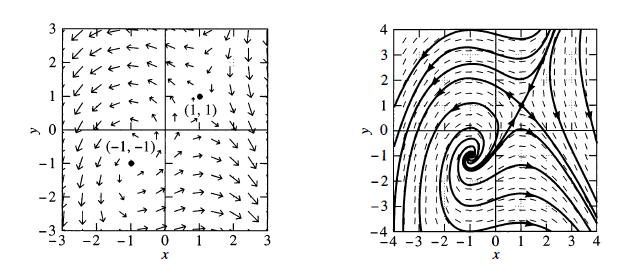
\includegraphics[width=15cm, height=6cm]{slope}
\end{center}
\captionof{figure}{En samling af linjeelementer(tv.) og et faseportæt(th.) til \eqref{DLS}. Figuren er taget fra \citep[s. 490]{EP}} \label{slope}
\hfill \break

\textnormal{På Figur \ref{slope} kan man se, hvordan løsningskurverne i faseportrættet følger linjeelementerne, og dermed også bevæger sig henholdsvis hen  imod eller væk fra ligevægtpunkterne.}

\end{Example}

\hfill \break
Vi karakteriserer ligevægtspunkter ud fra løsningskurvernes opførsel omkring dem. Givet et ligevægtspunkt $(x^*,y^*)$ i et autonomt system kaldes dette ligevægtspunkt således for en knude, såfremt følgende er gældene for løsningskurverne:
\begin{itemize}
    \item Enten går enhver løsningskurve mod ligevægtspunktet $(x^*,y^*)$ når $t \to + \infty$, eller også går enhver løsningskurve væk fra $(x^*,y^*)$ når $t \to + \infty$, og
    \item Enhver løsningskurve er tangent i $(x^*,y^*)$ til en lige linje igennem ligevægtspunktet.  
\end{itemize}
En knude kaldes en egentlig knude, hvis der ikke er et par af modsatliggende løsningskurver, der er tangent til den samme lige linje gennem $(x^*,y^*)$ og kaldes for en uegentlig knude, hvis dette ikke er tilfældet. Dette er illustreret i figur \ref{noder}.
\begin{figure} [H]
    \centering
    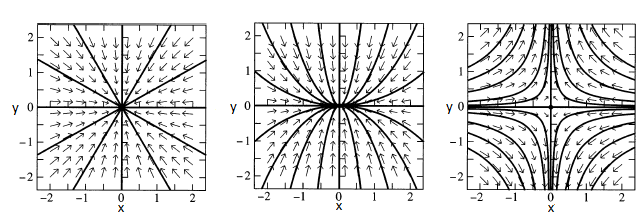
\includegraphics[scale=0.8]{Images/noder.png}
    \caption{En egentlig knude (tv.),en uegentlig knude (m) og et saddelpunkt (th.). Figuren er taget fra \citep[s. 491-492]{EP}}
    \label{noder}
\end{figure}

De to ligevægtspunkter til venstre i figur \ref{noder} kaldes også for dræn, da alle løsningskurverne går ind mod ligevægtspunktet. Hvis alle løsningskurverne går væk fra ligevægtspunktet, kaldes punktet en kilde.

Ligevægtspunktet yderst til højre i figur \ref{noder} kaldes et saddelpunkt. Et saddelpunkt er karakteriseret ved, at mindst en løsningskurve går mod $(x^*,y^*)$, at mindst en løsningskurve bevæger sig væk fra $(x^*,y^*)$ og, at de løsningskurver, der bevæger sig væk fra punktet, er ubegrænsede.
\\
En mere overordnet metode til beskrivelse af løsningskurvernes opførsel omkring et ligevægtspunkt, er ved brug af begrebet stabilitet.

\begin{definition}[Stabilitet af ligevægtspunkt]
Lad $\dot{y}(t)=\vec{f}(\vec{y(t)})$
være et autonomt differentialligningssystem, $\vec{y^*}=(y^*_{1},y^*_{2}, \cdots ,y^*_{n})$ et ligevægtspunkt og $\vec {y_0}=(y_{0,1},y_{0,2}, \cdots ,y_{0,n})$ et begyndelsespunkt. Ligevægtspunktet siges at være stabilt, såfremt der for ethvert $\varepsilon >0$ eksisterer et $\delta >0$ så følgende gælder:
$$|\vec y_0 - \vec {y^*}|< \delta \Rightarrow |\vec y(t) - \vec {y^*}| < \varepsilon, \\ \forall t > 0$$
\end{definition}
Et ligevægtspunkt kaldes ustabilt, hvis det ikke er stabilt.
Udover at være stabilt kan et ligevægtspunkt også være asymptotisk stabilt, hvilket vil sige, at det udover at være stabilt, også har egenskaben at alle løsningskurver tilstrækkelig tæt på ligevægtspunktet, vil bevæge sig ind mod ligevægtpunktet.

\begin{definition}[Asymptotisk stabilitet af ligevægtspunkt]
Lad 
$\dot{y}(t) = \vec{f}(\vec{y}(t))$
være et autonomt differentialligningssystem, $\vec {y^*}=(y_1^*,y_2^* \cdots ,y_n^*)$ et ligevægtspunkt og $\vec y_0=(y_{0,1},y_{0,2} \cdots ,y_{0,n})$ et begyndelsespunkt. Ligevægtspunktet siges at være asymptotisk stabilt, såfremt der eksisterer et $\delta >0$, så følgende gælder:
$$|\vec y_0 - \vec {y^*}|< \delta \Rightarrow \lim_{t\to\infty} \vec y(t)= \vec {y^*}$$
\end{definition}
Det ses således, at knuderne i figur \ref{noder} også kan beskrives som asymptotisk stabile ligevægtspunkter, mens saddelpunktet er ustabilt. \\
Et center er defineret ved, at alle løsningskurverne former lukkede kurver omkring centeret. Dette er et eksempel på et stabilt punkt, som ikke er asymptotisk stabilt, mens en spiral kan være enten asymptotisk stabil eller ustabil. Disse to tilfælde er illustreret i figur \ref{center}.

\begin{figure} [H]
    \centering
    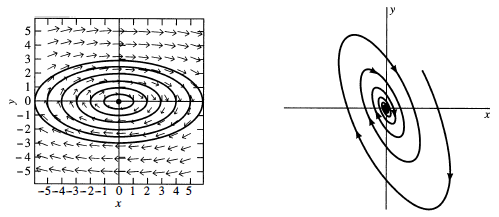
\includegraphics{Images/center.png}
    \caption{Et center (tv.) og en spiral (th.). Figuren er taget fra \citep[s. 493-495]{EP}}
    \label{center}
\end{figure}

\section{Stabilitets-analyse af system}
Dette afsnit samt underafsnit er baseret på \citep[afsnit 7.3]{EP} \\
Givet et autonomt system af differentialligninger,
\begin{equation}
\label{stab1}
    \begin{aligned}
    &\frac{dx}{dt}=F(x(t),y(t)),\\ 
    &\frac{dy}{dt}=G(x(t),y(t))
    \end{aligned}
\end{equation}
vil vi i dette afsnit undersøge, hvordan løsningerne opfører sig i nærheden af et isoleret ligevægtspunkt $(x^*,y^*)$. At et ligevægtspunkt er isoleret vil sige, at der i en omegn af ligevægtspunktet ikke eksisterer andre ligevægtspunkter. Det antages, at funktionerne $F$ og $G$ er kontinuerte og differentiable i en omegn af ligevægtspunktet.
Det kan antages uden tab af generalitet, at $x^*=y^*=0$. Dette kan med fordel antages, da vi
kun er interesseret i at sige noget om løsningskurvernes opførsel omkring ligevægtspunktet. Vi kan således omskrive systemet ved at sætte $u(t)=x(t)-x^*$ og $v(t)=y(t)-y^*$. Dermed bliver

\begin{equation*}
    \begin{aligned}
    &\frac{du}{dt}=\frac{dx}{dt}-\frac{dx^*}{dt}=\frac{dx}{dt}\\ 
    &\frac{dv}{dt}=\frac{dy}{dt}-\frac{dy^*}{dt}=\frac{dy}{dt},
    \end{aligned}
\end{equation*}

da $\frac{dx^*}{dt},\frac{dy^*}{dt}=0$. Systemet er dermed ækvivalent med det nye system:

\begin{equation}
\label{stab2}
    \begin{aligned}
    &\frac{du}{dt}=f(u(t),v(t)),\\ 
    &\frac{dv}{dt}=g(u(t),v(t))
    \end{aligned}
\end{equation}
hvor
\begin{equation*}
\begin{aligned}
&f(u,v)=F(u+x^*,v+y^*),\\ 
    &g(u,v)=G(u+x^*,v+y^*)
\end{aligned}
\end{equation*}
i den forstand at afbildningen, $(x(t),y(t)) \mapsto (u(t),v(t))$, definerer en bijektion af den ene løsningsmængde på den anden. Løsningskurverne for systemet $(\ref{stab1})$ er dermed lig løsningskurverne for $(\ref{stab2})$ efter koordinatskiftet $(u,v)\rightarrow(u+x^*,v+y^*)$. De to faseportrætter er altså identiske omkring de to ligevægtspunkter $(x^*,y^*)$ og $(0,0)$, som vist i figur (\ref{grafer}).
\begin{figure}[H]
    \centering
    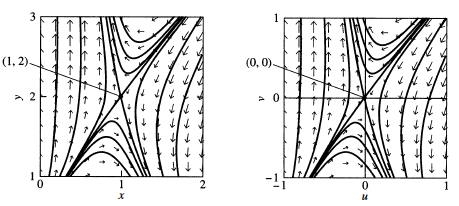
\includegraphics[scale=0.9]{grafer.png}
    \caption{System med ligevægtspunkt i $(1,2)$ i $x,y$-koordinatsystemet (th.) og det ækvivalente system i $u,v$-koordinatsystemet med ligevægtspunkt i $(0,0)$. Figuren er taget fra \citep[s. 501]{EP}}
    \label{grafer}
\end{figure}

\subsection{Linearisering}
Taylors formel for funktioner af to variable indebærer, at hvis funktionen $F(x,y)$ er kontinuert og differentiabel omkring punktet, $(x^*,y^*)$, så er jævnfør \citep[s. 501]{EP}:
\begin{equation*}
F(u+x^*,v+y^*)=F(x^*,y^*)+F_x(x^*,y^*)u+F_y(x^*,y^*)v+r(u,v),
\end{equation*}

hvor restledet $r(u,v)$ opfylder:
\begin{equation}
 \lim_{(u,v)\to (0,0)} \frac{r(u,v)}{\sqrt{u^2+v^2}}=0  
 \label{restled}
\end{equation}

Anvendes Taylors formel på funktionerne i det omskrevne system (\ref{stab2}), får vi funktionerne:

\begin{equation*}
    \begin{aligned}
    &F(u+x^*,v+y^*)=F(x^*,y^*)+F_x(x^*,y^*)u+F_y(x^*,y^*)v+r(u,v),\\ 
    &G(u+x^*,v+y^*)=G(x^*,y^*)+G_x(x^*,y^*)u+G_y(x^*,y^*)v+s(u,v),
    \end{aligned}
\end{equation*}
hvor $r(u,v)$ og $s(u,v)$  er restleddene. \\
Antag at, $(x^*,y^*)$, er et isoleret ligevægtspunkt. Så er,  $F(x^*,y^*)=G(x^*,y^*)=0$, og vi får:
\begin{equation*}
    \begin{aligned}
    &\frac{du}{dt}=F_x(x^*,y^*)u+F_y(x^*,y^*)v+r(u,v),\\ 
    &\frac{dv}{dt}=G_x(x^*,y^*)u+G_y(x^*,y^*)v+s(u,v)
    \end{aligned}
\end{equation*}

Da begge restled $r(u,v)$ og $s(u,v)$ opfylder ligning (\ref{restled}), vil vi altså, når $(u,v)$ er tæt på ligevægtspunktet $(0,0)$, få en tilnærmelse af det lineære system, som kan løses:

\begin{equation*}
    \begin{aligned}
    &\frac{du}{dt}=F_x(x^*,y^*)u+F_y(x^*,y^*)v,\\ 
    &\frac{dv}{dt}=G_x(x^*,y^*)u+G_y(x^*,y^*)v
    \end{aligned}
\end{equation*}
Dette lineariserede system vil således være en approksimation af det givne ikke-lineære system omkring ligevægtspunktet.
Det ses, at koefficienterne for $u$ og $v$ i det lineariserede system er henholdsvis $F_x(x^*,y^*),G_x(x^*,y^*)$ og $F_y(x^*,y^*),G_y(x^*,y^*)$. \\
Lineariseringen er altså givet ved:

\begin{equation*}
    \begin{aligned}
    &\frac{d\vec{u}}{dt}=\textbf{J}\vec{u}
    \end{aligned}
\end{equation*}
Hvor $\vec{u}=[u \ v]^T$ og $\textbf{J}$ er Jacobi-matricen for vektorfunktionen $(F,G)$ evalueret i ligevægtspunktet $(x^*,y^*)$. En Jacobi-matrix defineres ved:

\begin{definition}[Jacobi-matrix]
Lad $$\vec{f}: \mathbb{R}^n \to \mathbb{R}^m$$ være en funktion. \\ Da defineres en $m \times n$ matrix, $\textbf{J}$, på $\vec{f}$ til at være Jacobi-matricen til funktionen og skrives på formen:
$$\textbf{J}_{\vec{f}}(\vec{y}) = \frac{d\vec f}{d\vec{y}} =
\begin{bmatrix}
    \frac{\partial f_1}{\partial y_{1}} & \frac{\partial f_1}{\partial y_{2}} & \dots & \frac{\partial f_1}{\partial y_{n}} \\
    \frac{\partial f_2}{\partial y_{1}} & \frac{\partial f_2}{\partial y_{2}} & \dots & \frac{\partial f_2}{\partial y_{n}} \\
    \vdots & \vdots & \ddots & \vdots \\
    \frac{\partial f_m}{\partial y_{1}} & \frac{\partial f_m}{\partial y_{2}} & \dots & \frac{\partial f_m}{\partial y_{n}}
\end{bmatrix},$$
eller komponentvist:
$$\textbf{J}_{ij} = \frac{\partial f_i}{\partial y_j}$$

Jacobi-matricen er en lineær afbildning $\mathbb{R}^n \to \mathbb{R}^m$, der angiver en lineær approksimation af $\vec{f}$ til et $\vec{y}$.
\end{definition}

\subsection{Analyse af lineære systemer}\label{AnalLinSys}

Givet et lineært system af differentialligninger på formen,
$$\dot{y}(t) = A \vec{y}(t)$$
kan vi ved hjælp af egenværdierne for matricen $A$ analysere ligevægtspunkterne i systemet. \\ 
Givet et lineært system af differentialligninger i $\mathbb{R}^2$ findes egenværdierne, af koefficient matricen $A$, ved at løse den karakteristiske ligning:

\begin{equation}
 \det(A-\lambda I)= \begin{vmatrix}
a-\lambda & b \\
c & d -\lambda
\end{vmatrix}=(a-\lambda)(d-\lambda)-bc=0
\label{detA}
\end{equation}
Lad $(0,0)$ være et isoleret ligevægtspunkt, så vil $\det A$ være forskellig fra $0$, da ligevægtspunktet kun er isoleret, såfremt matricen $A$ er invertibel, og den homogene ligning dermed kun har den trivielle løsning $(0,0)$.\\
Dette betyder, at $\lambda=0$ ikke er en løsning i \eqref{detA}. Dermed er begge egenværdier for $A$ forskellige fra $0$.

De to egenværdier kan altså være:
\begin{itemize}
    \item Reelle og forskellige med samme fortegn
    \item Reelle og forskellige med forskelligt fortegn
    \item Reelle og ens
    \item Kompleks konjugerede med real-del forskellig fra 0
    \item  Rent imaginære
\end{itemize}

\subsubsection{Reelle og forskellige med samme fortegn}
I dette tilfælde har matricen $A$ to lineært uafhængige egenvektorer $\vec{v_1}$ og $\vec{v_2}$. Den fuldstændige løsning kan dermed skrives som:
$$\vec{y}(t)=c_1\vec{v_1}e^{\lambda_1 t}+c_2\vec{v_2}e^{\lambda_2 t}$$
Betragtes denne løsning i et $uv$-koordinatsystem med $\vec{v_1}$ og $\vec{v_2}$ som basisvektorer, som vist i figur \ref{uv-koordinatsystem}, vil en løsningskurve, som opfylder begyndelsesbetingelserne $u(0)=u_0$ og $v(0)=v_0$ kunne beskrives ved:
\begin{equation*}
    u(t)=u_0e^{\lambda_1 t} \ \  v(t)=v_0e^{\lambda_2 t}
\end{equation*}
\begin{figure}[H]
    \centering
    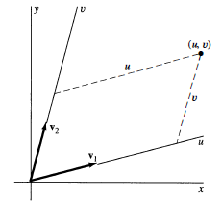
\includegraphics[scale=0.9]{uv-koordinatsystem.png}
    \caption{$u,v$-koordinatsystemet bestemt ved egenvektorerne $\vec{v_1}$ og $\vec{v_2}$ \citep[s. 503]{EP}}
    \label{uv-koordinatsystem}
\end{figure}
Hvis $v_0=0$ eller $u_0=0$ vil løsningskurven ligge på henholdsvis $u$-aksen og $v$-aksen. Hvis $u_0,v_0 \neq 0$ kan den parametriske kurve skrives på formen $v=Cu^k$. Dette ses ved følgende udregning:
\begin{equation*}
    u(t)=u_0e^{\lambda_1 t} \Rightarrow \ln \left(\frac{u(t)}{u_0} \right)=\lambda_1 t \Rightarrow t= \frac{\ln \left(\frac{u(t)}{u_0} \right)}{\lambda_1}
\end{equation*}
Foregående udregning kan foretages, da $u(t)$ og $u_0$ altid har samme fortegn, da $e^{\lambda_1 t} > 0$.
\begin{equation*}
v(t)=v_0e^{\lambda_2 t}=v_0e^{\lambda_2 \frac{\ln \left(\frac{u(t)}{u_0} \right)}{\lambda_1}} =  v_0\left(\frac{u(t)}{u_0}\right)^{\frac{\lambda_2}{\lambda_1}}
\end{equation*}
Altså er $v=Cu^k$, hvor $C=\frac{v_0}{u_0^{(\lambda_2 / \lambda_1)}}$ og $k=\frac{\lambda_2}{\lambda_1} > 0$, da egenværdierne har samme fortegn. \\
Da $v=Cu^k$ er en potensfunktion, vil løsningskurven være  tangent med $v$-aksen i $(0,0)$ for $k>1$, og for $0<k<1$ er den tangent med $u$-aksen. $(0,0)$ er derfor en uegentlig knude. Hvis egenværdierne er positive, vil løsningskurverne bevæge sig væk fra ligevægtspunktet, når $t \to \infty$. $(0,0)$ er derfor en kilde i dette tilfælde. Det modsatte gør sig gældende, hvis begge egenværdier er negative, i hvilket tilfælde $(0,0)$ vil være et dræn.
\subsubsection{Reelle og forskellige med forskelligt fortegn}
Som i forrige tilfælde kan løsningskurverne bestemmes ved:
\begin{equation*}
    u(t)=u_0e^{\lambda_1 t} \ \  v(t)=v_0e^{\lambda_2 t}
\end{equation*}
Forskellen er nu bare at $\lambda_2<0<\lambda_1$. Løsningskurverne, hvor $u_0,v_0 \neq 0$, kan som før skrives på formen $v=Cu^k$, hvor forskellen er, at $k=\frac{\lambda_2}{\lambda_1}<0$. Løsningskurverne vil derfor være hyperbler, og ligevægtspunktet er dermed ustabilt.
\subsubsection{Reelle og ens}
I dette tilfælde afhænger opførslen af løsningskurverne omkring ligevægtspunktet af, om $A$-matricen har to lineært uafhængige egenvektorer. Hvis dette er tilfældet kan løsningskurverne som før beskrives ved $v=Cu^k$ i $uv$-koordinatsystemet, hvor $k=1$ i dette tilfælde. Vi får dermed $v=Cu$, og løsningskurverne ligger altså på en lige linje gennem origo. Ligevægtspunktet vil derfor være en egentlig knude. Hvis $\lambda>0$ er punktet en kilde, og hvis $\lambda<0$ er punktet et dræn. \\
Hvis $A$-matricen ikke har to lineært uafhængige egenvektorer, har systemet to lineært uafhængige løsninger:
\begin{equation*}
    \vec{y_1}(t)=\vec{v_1}e^{\lambda t} \ \textnormal{og} \ \vec{y_2}(t)=(\vec{v_1}t+\vec{v_2})e^{\lambda t}
\end{equation*}
Og dermed den fuldstændige løsning:
\begin{equation*}
    c_1\vec{y_1}(t)+c_2\vec{y_2}(t) = \\
    (c_1+c_2t)\vec{v_1}e^{\lambda t} +c_2\vec{v_2}e^{\lambda t}
\end{equation*}
Hvor $\lambda$ er systemets egenværdi med tilhørende egenvektore $\vec{v_1}$, og $\vec{v_2}$, som opfylder $(A-\lambda I)\vec{v_2}=\vec{v_1}$.
Som før kan løsningskurverne beskrives i et $uv$-koordinatsystem bestemt af $\vec{v_1}$ og $\vec{v_2}$. Løsningskurverne kan altså beskrives ved:
\begin{equation*}
    v(t)=v_0e^{\lambda t}, \ u(t)=(u_0+v_0t)e^{\lambda t}
\end{equation*}
Hvor $v_0=v(0)$ og $u_0=u(0)$. Hvis $v_0=0$ ligger løsningskurven på $u$-aksen. Ellers gælder følgende for løsningskurven:
\begin{equation*}
    \frac{dv}{du}=\frac{\frac{dv}{dt}}{\frac{du}{dt}}=\frac{\lambda v_0e^{\lambda t}}{v_0e^{\lambda t}+\lambda(u_0+v_0t)e^{\lambda t}}=\frac{\lambda v_0}{v_0+\lambda(u_0+v_0t)}
\end{equation*}
Det ses at $\frac{dv}{du} \to 0$ nåt $t \to \pm
\infty$. Altså er enhver løsningskurve tangent med $u$-aksen. $(0,0)$ er derfor en uegentlig knude. Den er en kilde, hvis $\lambda>0$ og et dræn, hvis $\lambda<0$.
\subsubsection{Kompleks konjugerede med real-del forskellig fra 0}
Hvis systemet har to komplekst konjugerede egenværdier $\lambda = p+qi$ og $\bar{\lambda}=p-qi$, (hvor $p,q \neq 0$) med tilhørende komplekst konjugerede egenvektorer $\vec{v}=\vec{a}+\vec{b}i$ og $\bar{\vec{v}}=\vec{a}-\vec{b}i$. Så har systemet to uafhængige løsninger:
\begin{equation*}
    \vec{y_1}(t)=e^{pt}(\vec{a}\cos(qt)-\vec{b}\sin(qt)) \ \textnormal{og} \ \vec{y_2}(t)=e^{pt}(\vec{b}\cos(qt)+\vec{a}\sin(qt))
\end{equation*}
Den fuldstændige løsning er altså givet ved:
\begin{equation*}
    \vec{y}(t)=c_1e^{pt}(\vec{a}\cos(qt)-\vec{b}\sin(qt))+c_2e^{pt}(\vec{b}\cos(qt)+\vec{a}\sin(qt))
\end{equation*}
Hvilket kan omskrives til:
\begin{equation*}
    \vec{y}=\begin{bmatrix}
        \vec{a} & \vec{b}
    \end{bmatrix} \begin{bmatrix}
        \cos(qt) & \sin(qt) \\
        -\sin(qt) & \cos(qt)
    \end{bmatrix} \begin{bmatrix}
        c_1e^{pt} \\
        c_2e^{pt}
    \end{bmatrix}
\end{equation*}
Hvis $p<0$ vil  $c_1e^{pt},c_2e^{pt} \to 0$ når $t \to +\infty$. Da vektoren $\begin{bmatrix}
        c_1e^{pt} \\
        c_2e^{pt}
    \end{bmatrix}$ ganges på en rotationsmatrix, er $(0,0)$ i dette tilfælde et spiral dræn. Hvis $p>0$, vil ligevægtspunktet være en spiral kilde. Dette skyldes, at vi får en cirkel, for $t$ gennemløbende $[0,\frac{2\pi}{q}]$, hvis $e^{pt}$ udelades fra formlen. 
\subsubsection{Rent imaginære}
Hvis systemet har kompleks konjugerede egenværdier $\lambda=qi$ og $\bar{\lambda}=-qi$ med tilhørende kompleks konjugerede egenvektorer $\vec{v}=\vec{a}+\vec{b}i$ og $\bar{\vec{v}}=\vec{a}-\vec{b}i$. Så har systemet samme løsning som i forrige afsnit, hvor $p=0$:
\begin{equation*}
    \vec{x}(t)=c_1(\vec{a}\cos(qt)-\vec{b}\sin(qt))+c_2(\vec{b}\cos(qt)+\vec{a}\sin(qt))
\end{equation*}
Som før kan dette omskrives til:
\begin{equation*}
    \vec{x}(t)=\begin{bmatrix}
        \vec{a} & \vec{b}
    \end{bmatrix} \begin{bmatrix}
        \cos(qt) & \sin(qt) \\
        -\sin(qt) & \cos(qt)
    \end{bmatrix} \begin{bmatrix}
        c_1\\
        c_2
    \end{bmatrix}
\end{equation*}
Vi kan omskrive udtrykket for $\vec{x}(t)$ ved først at lave to omskrivninger af udtrykkende $c_1\cos(qt)+c_2\sin(qt)$ og $-c_1\sin(qt)+c_2\cos(qt)$:
\begin{equation*}
    c_1\cos(qt)+c_2\sin(qt)=\begin{pmatrix}
        c_1 \\ c_2
    \end{pmatrix} \cdot \begin{pmatrix}
        \cos(qt) \\ \sin(qt) 
    \end{pmatrix}  = \sqrt{c_1^2+c_2^2}\begin{pmatrix}
        \frac{c_1}{\sqrt{c_1^2+c_2^2}}\\ \frac{c_2}{\sqrt{c_1^2+c_2^2}}
    \end{pmatrix} \cdot \begin{pmatrix}
        \cos(qt) \\ \sin(qt) 
    \end{pmatrix}
\end{equation*}
Da $\begin{pmatrix}
        \frac{c_1}{\sqrt{c_1^2+c_2^2}}\\ \frac{c_2}{\sqrt{c_1^2+c_2^2}}
    \end{pmatrix}$ er en enhedsvektor, kan vi omskrive til følgende:
\begin{equation*}
\sqrt{c_1^2+c_2^2}\begin{pmatrix}
        \frac{c_1}{\sqrt{c_1^2+c_2^2}}\\ \frac{c_2}{\sqrt{c_1^2+c_2^2}}
    \end{pmatrix} \cdot \begin{pmatrix}
        \cos(qt) \\ \sin(qt) 
    \end{pmatrix}=
     \sqrt{c_1^2+c_2^2}\begin{pmatrix}
        \cos(\alpha)\\ 
        \sin(\alpha)
    \end{pmatrix} \cdot \begin{pmatrix}
        \cos(qt) \\ \sin(qt) 
    \end{pmatrix}
\end{equation*}
Da $\vec{a} \cdot \vec{b}= ||\vec{a}|| \ ||\vec{b}||\cos(\theta)$, hvor $\theta$ er vinklen mellem de to vektorer, får vi: 
\begin{equation*}
    \sqrt{c_1^2+c_2^2}\begin{pmatrix}
        \cos(\alpha)\\ 
        \sin(\alpha)
    \end{pmatrix} \cdot \begin{pmatrix}
        \cos(qt) \\ \sin(qt) 
    \end{pmatrix}=\sqrt{c_1^2+c_2^2}\cos(qt-\alpha)
\end{equation*} 
På samme måde kan vi finde et udtryk for $-c_1\sin(qt)+c_2\cos(qt)$, men udregningerne vil ikke blive gennemgået igen. Vi får udtrykket:
\begin{equation*}
    -c_1\sin(qt)+c_2\cos(qt)= \sqrt{c_1^2+c_2^2}\sin(qt-\alpha)
\end{equation*}
Vi kan nu udtrykke $\vec{x}(t)$ som følger:
\begin{equation*}
    \vec{x}(t)=\sqrt{c_1^2+c_2^2}\cos(qt-\alpha)\vec{a}+\sqrt{c_1^2+c_2^2}\sin(qt-\alpha)\vec{b}
\end{equation*}
\\
Det ses altså, at i dette tilfælde vil løsningskurven være en ellipse med $(0,0)$ som centrum, da vektorerne $\vec{a}$ og $\vec{b}$ ikke har samme længde. Dermed er $(0,0)$ et stabilt centrum i dette tilfælde. \\

Ovenstående afsnit opsummeres i en tabel: 

\begin{table} [H]
\centering 
    \begin{tabular}{|l|l|l|}
    \hline
    \textbf{Egenværdier}                                    & \textbf{Type af ligevægtspunkt}            & \textbf{Stabilitet}          \\ \hline
    $\lambda_1 > \lambda_2 > 0$                     & Uegentlig kilde                   & Ustabilt            \\ \hline
    $\lambda_1 < \lambda_2 < 0$                     & Uegentlig dræn                    & Asymptotisk stabilt \\ \hline
    $\lambda_1 < 0 < \lambda_2$                     & Saddelpunkt                       & Ustabilt            \\ \hline
    $\lambda_1 = \lambda_2 > 0$                     & Egentlig eller uegentlig kilde    & Ustabilt            \\ \hline
    $\lambda_1 = \lambda_2 < 0$                     & Egentlig eller uegentlig dræn     & Asymptotisk stabilt \\ \hline
    $\lambda_1, \lambda_2 =p \pm qi, p > 0$         & Spiralkilde                       & Ustabilt            \\ \hline
    $\lambda_1, \lambda_2 =p \pm qi, p < 0$         & Spiraldræn                        & Asymptotisk stabilt \\ \hline
    $\lambda_1, \lambda_2 = \pm qi, q > 0$          & Centrum                           & Stabilt             \\ \hline
    \end{tabular}
\caption{Sammenhæng mellem egenværdier og ligevægtspunkter}\label{tab:egenvardi}
\end{table}

\textbf{Bemærk} at jævnfør \citep[s. 738]{FDEB}, vil tabellen for egenværdierne for et lineariseret system være den samme, dog med undtagelse af de tilfælde hvor egenværdierne er reelle og ens, eller rent imaginære. For tilfældet hvor egenværdierne er reelle og ens vil løsningskurverne ligeledes kunne danne spiralpunkt. I tilfældet hvor egenværdierne er rent imaginære vil ligevægtspunktet være et centrum eller spiralpunkt og være enten stabilt, ustabilt eller asymptotisk stabilt. For det lineariserede system, i form af Jacobi-matricen, vil det altså ikke være tilstrækkeligt at benytte egenværdierne til at beskrive ligevægtspunktet. I disse tilfælde vil der i projektet anvendes Lyapunov-funktioner for yderligere analyse af stabiliteten af ligevægtspunktet.



